\subsection{Real Robot Table Tennis}

In this section we describe and discuss our experiments on the robotic table tennis setup, see Figure~\ref{robot}. 
%We have used a graphical simulation environment to evaluate our algorithm in Table~\ref{tableSimResults}. The realistic simulation platform is designed to imitate the features of our robotic table tennis setup, see Figure~\ref{robot}. 

\paragraph{\textbf{Description of the Setup}.} Our robot is a seven degree of freedom Barrett WAM arm that can easily reach $10g$ m/$\textrm{s}^2$ accelerations. It is torque-controlled and cable-driven. A standard size racket ($7.6$ cm radius) is attached to the end-effector. The vision system tracks the balls at a rate of $60$ Hz and consists of four cameras on the corners on the ceiling. See~\citet{Lampert12} for platform details. The table and the tennis balls are standard sized, the balls have a radius of $2$ cm, the table geometry is approximately $276 \times 152 \times 76$ cm.

%Even though the cameras are capable of $200$ Hz monitoring, expensive debayering and filtering operations reduce the tracking to around $60$ Hz range.

In the robot experiments, we use a ball-launcher (see Figure~\ref{robot}) to throw balls to the the robot, approximately once every $2-3$ seconds. The balls generally come with a high variance, especially the velocities are quite unpredictable even without oscillating the ball-launcher. The robot base is at a distance of $115$ cm to the end of the table and $95$ cm above the table. Robot base is centered with respect to the table in the $x$ direction, see Figure~\ref{robot}. %The robot's forehand posture $\joint_0$ is chosen the same as in our simulations. 
%
\begin{figure}
	\begin{subfigure}[t]{0.5\textwidth}
		\centering
		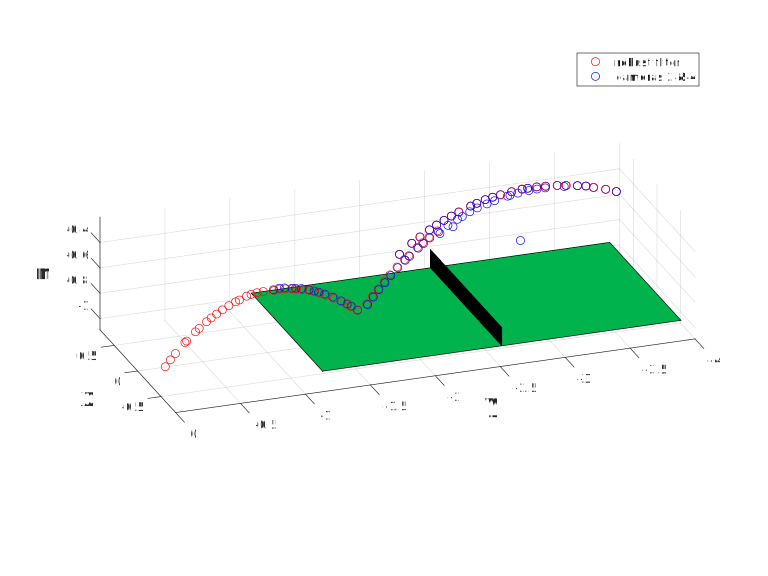
\includegraphics[scale=0.4]{robust_filtering_cam3.pdf}
		\caption{Filtering the noisy and corrupted data acquired from cameras 3 and 4 opposite to the robot side.}
		\label{outliersDataCam3}
	\end{subfigure}
	~ % remove this when using two column format
	\begin{subfigure}[t]{0.5\textwidth}
		\centering
		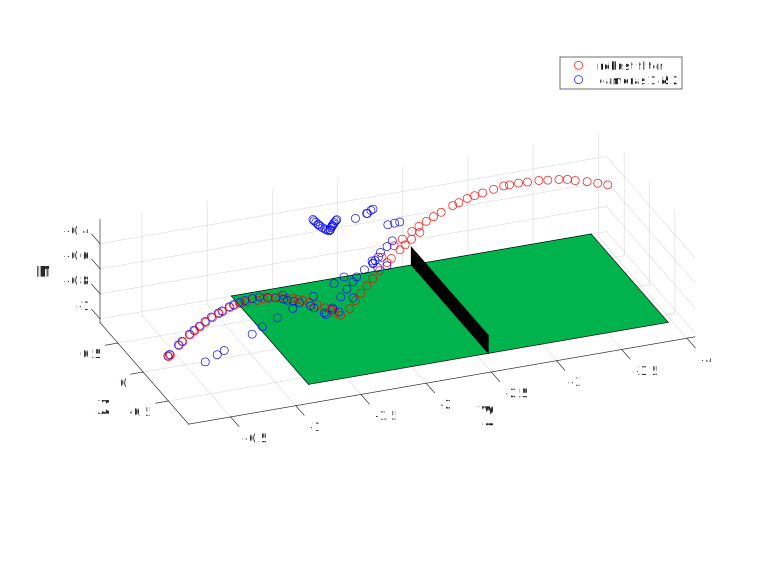
\includegraphics[scale=0.4]{robust_filtering_cam1.pdf}
		\caption{Filtering the noisy and corrupted data acquired from cameras 1 and 2 on the robot side.}
		\label{outliersDataCam1}
	\end{subfigure}
	\caption{Kalman Filtering with simultaneous outlier detection. The ball detection algorithm sometimes outputs outliers, typically more as the ball approaches the racket. Such corrupted data can be identified and discarded using the covariance of the Kalman Filter.}
	\label{outliersData}
\end{figure}
%
\paragraph{\textbf{Estimation and Outlier Detection}.} The ball detection algorithm detects the center of mass of the orange balls from each image separately and fuses them together to form two ball position estimates. These are then preprocessed and filtered with an Extended Kalman Filter (EKF) to estimate ball position and velocity. 

After the ball-launcher shoots a ball, $\numBallsMin \approx \minball$ ball observations are used to initialize the Kalman Filter state and launch the trajectory generation process, see Algorithms~\ref{alg1} and \ref{alg2}. Balls that suddenly appear on the opponent's court after disappearing for more than $\resetTime$ seconds from the cameras cause the Kalman Filter to reset. The filter state and the ball spin (assumed constant throughout motion) are then estimated together with a truncated Newton's method~\footnote{The optimization is launched on another thread using the \emph{TNEWTON} algorithm in NLopt~\citep{NLopt}.} using $\numBallsMin = \minball$ ball samples. We have experimentally confirmed the value of $\numBallsMin$ to be a good compromise between ball estimation accuracy (which requires waiting) and moving early (which can reduce the accelerations).
% TODO: plot here to show the trade-off curve

% RESETTING IS NOT MENTIONED IN THE ALGORITHMS - PUT A SUBBLOCK ?
The ball detection algorithm sometimes outputs outliers, possibly meters away from the actual ball. This typically happens more as the ball approaches the racket and new ball observations become more valuable. In order to prevent the outliers from ruining the estimation and the overall performance, we have implemented a robust EKF that does not perform measurement updates, if the ball observations lie more than $2$ standard deviations away from the predicted state. See Figure~\ref{outliersData} for actual table tennis ball data.
%
% PUT HERE AN EQUATION FOR OUTLIER DETECTION
%
We adjust the covariance estimates $\vec{\Sigma}(t)$ accordingly to make this procedure work in practice, e.g., covariances are initialized with a large $\vec{\Sigma}_{\mathrm{init}}$ value and the noise covariances $\vec{W}(t) \approx \diag(10^{-3})$ are adjusted to make sure that $\vec{\Sigma}(t)$ decreases suitably over time.
%
%Running the optimizers repeatedly allows us to correct for prediction and control errors, as in Model Predictive Control~\citep{Garcia89}.
%
%
\paragraph{\textbf{Online Correction of Computed Trajectories}.} Since the ball is moving at fast speeds, our online trajectory generation algorithms needs to be on the order of tens of milliseconds, in order to reliably intercept the incoming ball. The optimizers take on average $20-25$ ms to converge, and they can be re-run in the real-time platform whenever there are new reliable ball observations $\ball_\mathrm{obs}$. Before launching the trajectory optimizers, the path of the ball is predicted each time for $\predTime = 1.0$ seconds and the algorithms are initialized with current joint state estimates $\joint_{\textrm{cur}}, \dot{\joint}_{\textrm{cur}}$. During this correction process, we make sure that the updates are always incremental and feasible. For completeness, we list here our software checks. We make sure that:
%
\begin{enumerate}
	\item At least $N = \minball$ reliable ball observations are available. This typically happens before the balls pass the net.
	\item The new ball estimate is not too far off from the previous estimates.
	\item Our previous optimization thread has terminated before another one is launched.
	\item The resulting Cartesian trajectory intersects with the ball and all the task constraints are satisfied.
	\item The corrections are never excessive, i.e., the acceleration and joint limits \eqref{jointLimPointwise} and \eqref{jointLimTraj} are always respected.
	\item The ball estimate appears to be in front of the robot, i.e., $b_y < r_y$.
\end{enumerate}
%
If any of these conditions are violated, then the trajectories are not updated, and the previous striking trajectory is followed without interruption. 
%
%
The balls come with a high variance in position and especially in velocity. Typical incoming ball velocities imparted by the ball-launcher are around $4-6$ m/s range in the y-direction, which implies that in practice there can be a maximum of $10$ ball corrections till the ball passes the robot. The ball-launcher gives in addition a lot of $\emph{topspin}$ to the ball. This makes the corrections provided by the repeated optimization critical, as the ball models~\mbox{\eqref{flightModel} -- \eqref{contactModel}} are unable to capture some of the aerodynamic effects due to spin. Figure~\ref{predErrorReduction} shows the decrease in mean squared prediction error as more ball observations are acquired.
%
\begin{figure}
	\centering
	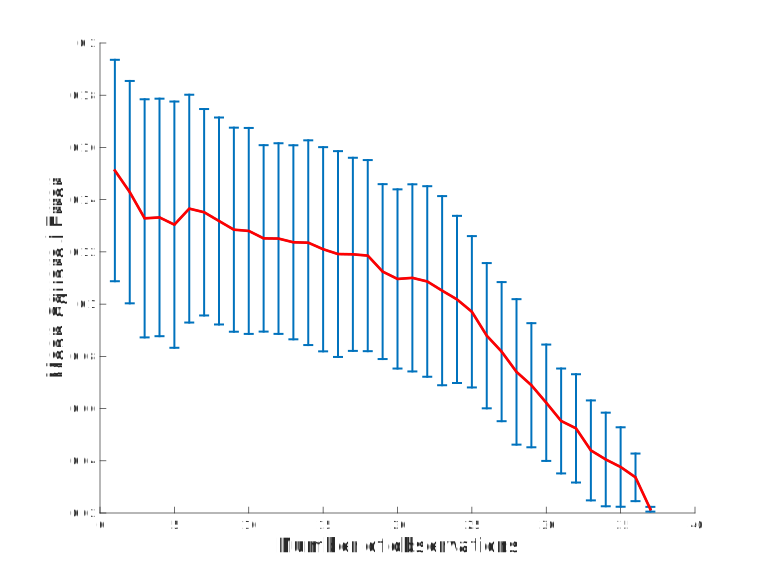
\includegraphics[scale=0.4]{predErrorReductionSpin.pdf}
	\caption{Mean squared prediction error (red curve) is reduced as more balls are observed. The ball observations are used until contact with racket occurs and the results are averaged over $100$ different real ball trials. Correcting for ball prediction error is critical for a robust table tennis performance, as the balls typically come with a high spin. Balls seems to lose some spin after rebound and the prediction error decreases faster. In this case this phenomenon can be observed after about $25$ ball observations, where the change in the average slope of the red curve can be seen.}
	\label{predErrorReduction}
\end{figure}
%
%topspin - roughly at $3000$ rates per minute
%
%Two example Cartesian trajectories computed by $\Alg$ are shown in Figure~\ref{fig:0} and Figure~\ref{fig:3}. The figures are snapshots of our simulation platform. Resulting trajectories naturally incorporate a swingback motion whenever needed, without explicit programming. More natural strikes can be computed in our framework. In the case shown in Figure~\ref{fig:0} for example, setting a VHP in front of the robot would result in very high accelerations, whereas the computed optimal trajectory intercepts with the ball trajectory behind the initial pose of the robot.
%
%\begin{figure}
%  \begin{subfigure}[t]{0.45\textwidth}
%    \centering
%    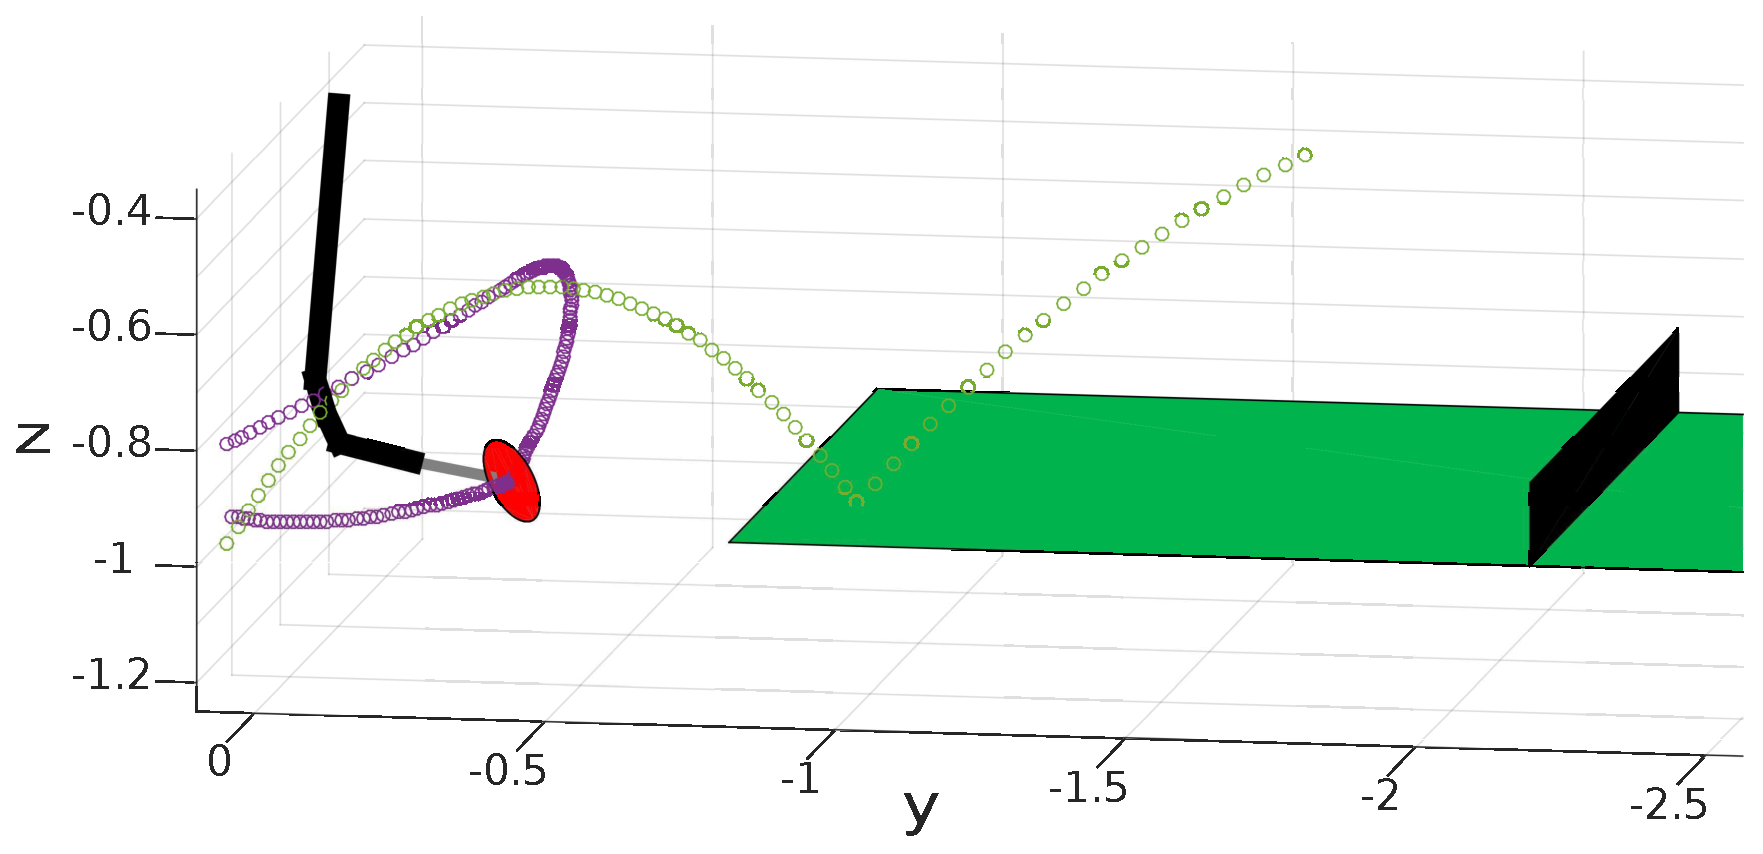
\includegraphics[width=\textwidth]{racket_ball_traj_0.eps}
%    \caption{Rest posture}
%    \label{fig:1}
%  \end{subfigure}
%  ~ % remove this when using two column format
%  \begin{subfigure}[t]{0.45\textwidth}
%  	\centering
%    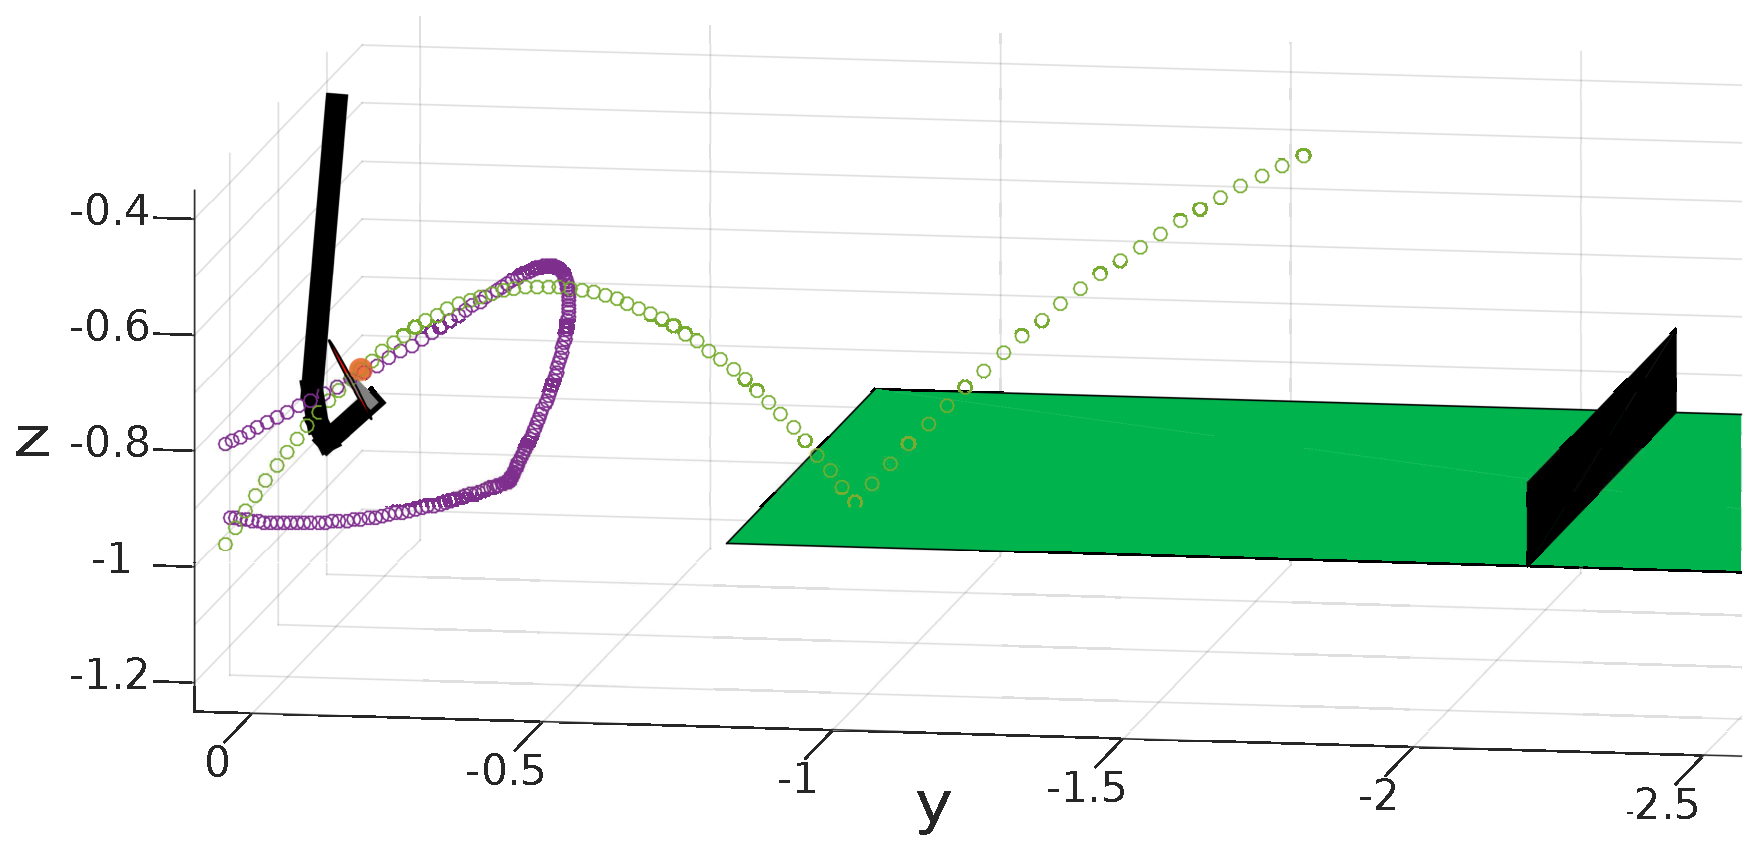
\includegraphics[width=\textwidth]{racket_ball_traj_1.eps}
%    \caption{Posture at striking time}
%    \label{fig:2}
%  \end{subfigure}
%  \caption{An example trajectory generated by the optimal control based framework is shown in purple. The resulting trajectory, minimizing the accelerations throughout, incorporates naturally a swingback pattern that may not be included in other methods fixing a virtual hitting plane (VHP).}
%  \label{fig:0}
%\end{figure}
%
%\begin{figure}[t!]
%\centering
%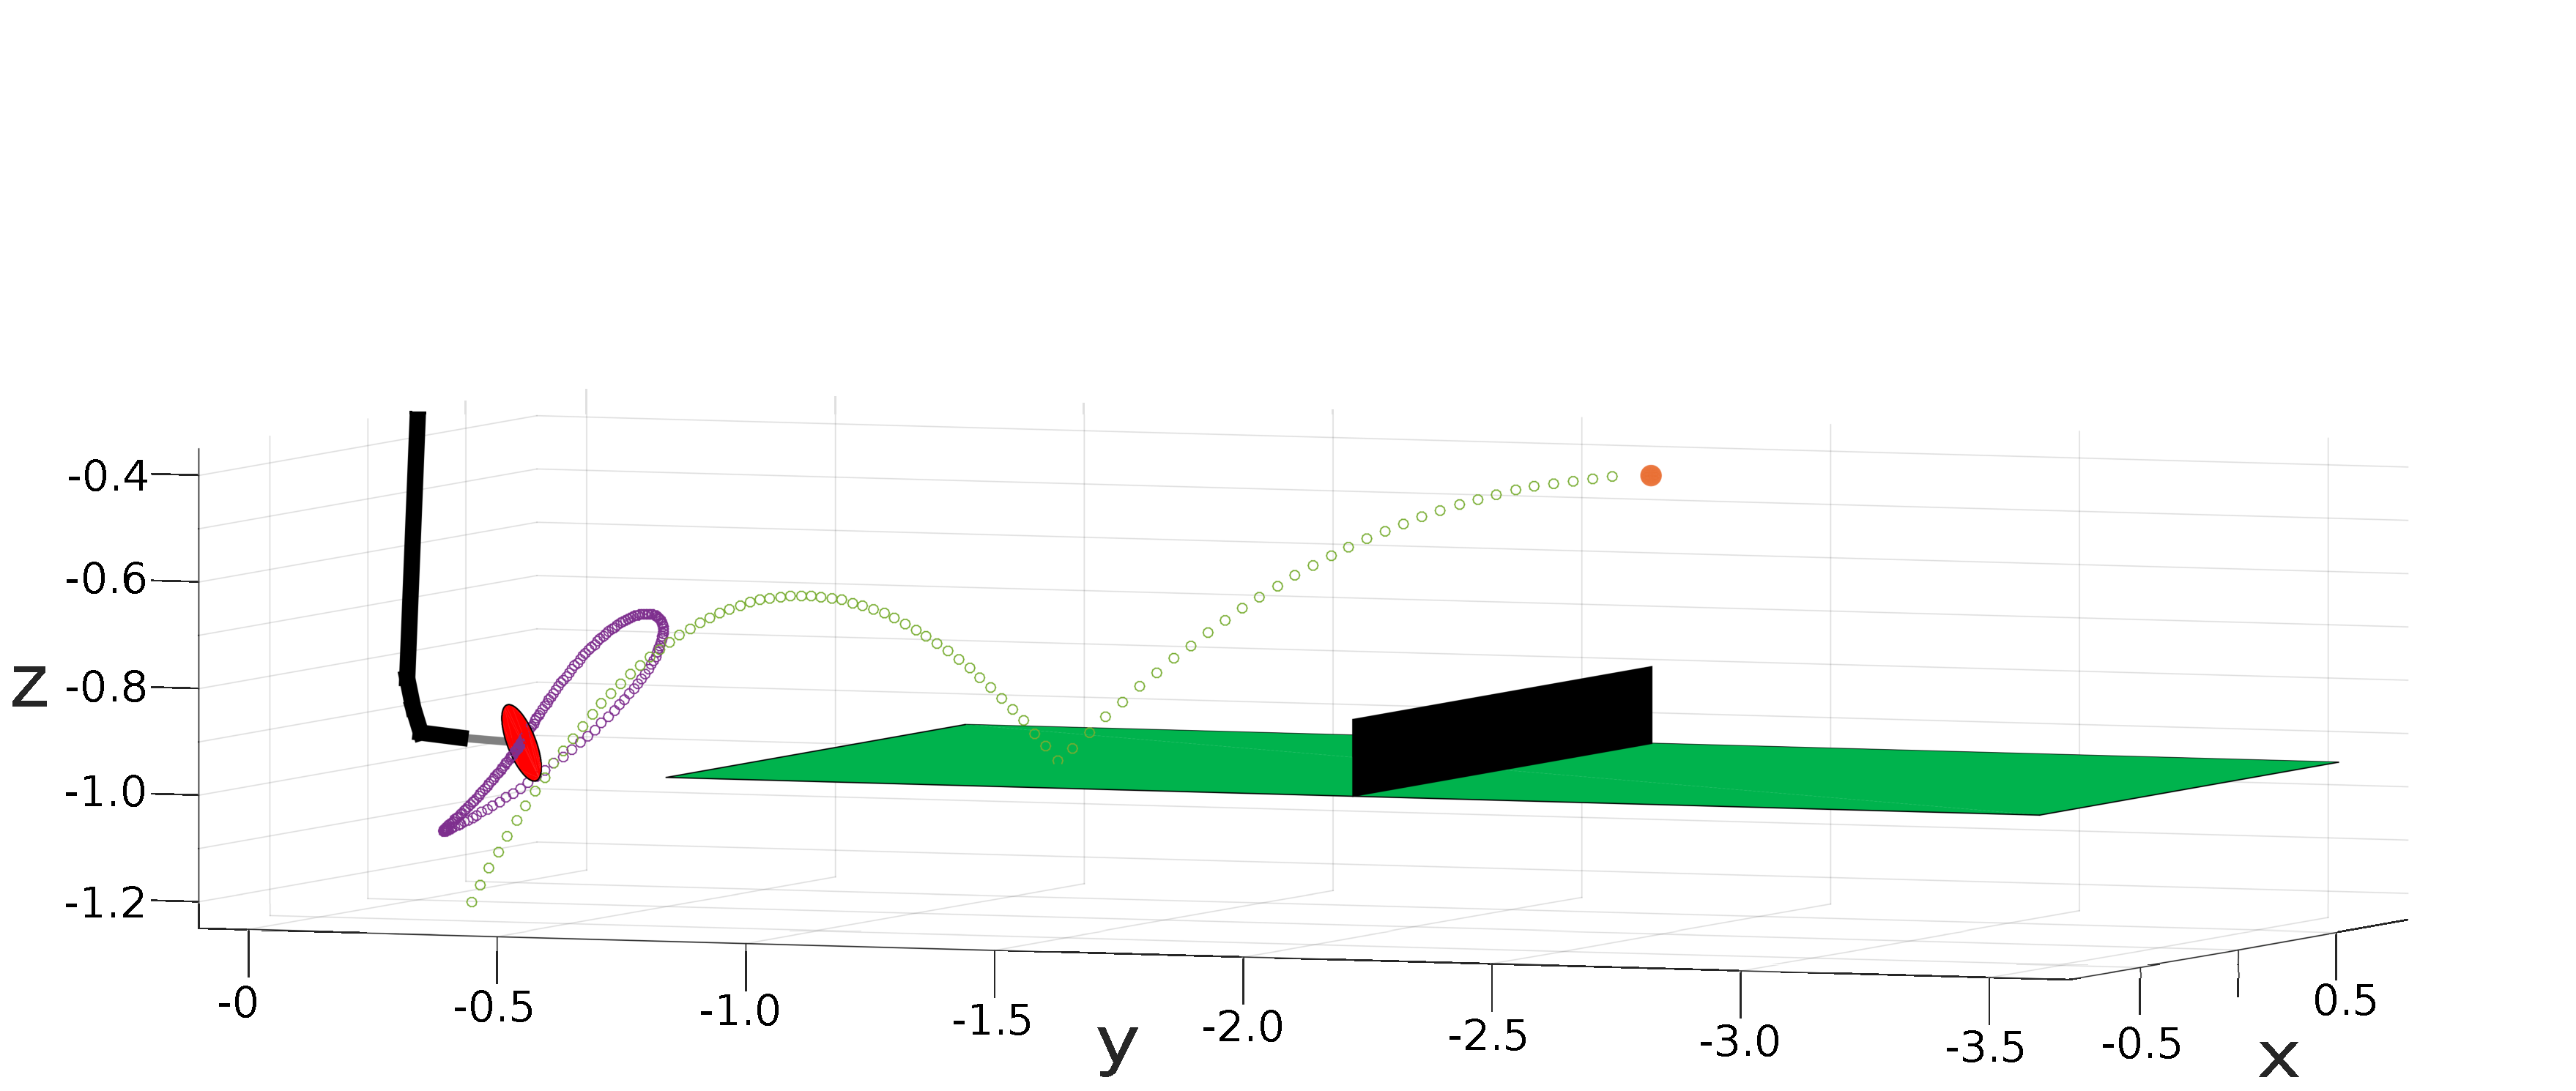
\includegraphics[scale=0.15]{racket_ball_traj_2.eps}	
%\caption{Another computed optimal trajectory. In this case, there is less swingback and the alignment with the ball trajectory is higher.}
%\label{fig:3}
%\end{figure}
%
\paragraph{\textbf{Discussion of Results}.} We compare and evaluate the performance of the two players $\alg$ and $\algTwo$ in the robot table tennis setup, see Figures~\ref{compare-players-real} and~\ref{exampleTT}. Results are averaged over $200$ trials where the ball-launcher is fixed at different positions or is oscillating, and the robot is placed at three different initial postures. For $\alg$, we also consider the variation in performance due to selecting different desired landing positions and landing times. Overall, $\alg$ is able to return about $40-60 \%$ of the balls to the opponent's court. Setting the desired landing position on the right side of the table, with a desired landing time of $T_{\textrm{land}} = 0.4$ seconds, leads to the best performance ($\sim 60\%$) in our table tennis setup. Increasing the time and setting the desired landing position closer to the centre of the opponents court makes the player less robust, decreasing the accuracy down to $40-50\%$ and increasing the variance of the landing locations, see Figure~\ref{distr_returns}. We believe this decrease in the performance is due to inaccuracies in the racket model.
%
% 
\begin{figure}
	\centering
	\setlength\figureheight{4cm}
	\setlength\figurewidth{5cm}
	% This file was created by matlab2tikz.
%
%The latest updates can be retrieved from
%  http://www.mathworks.com/matlabcentral/fileexchange/22022-matlab2tikz-matlab2tikz
%where you can also make suggestions and rate matlab2tikz.
%
\definecolor{mycolor1}{rgb}{0.20810,0.16630,0.52920}%
\definecolor{mycolor2}{rgb}{0.21783,0.72504,0.61926}%
\definecolor{mycolor3}{rgb}{0.97630,0.98310,0.05380}%
\definecolor{mycolor4}{rgb}{0.00000,0.44700,0.74100}%
%
\begin{tikzpicture}

\begin{axis}[%
width=0.951\figurewidth,
height=\figureheight,
at={(0\figurewidth,0\figureheight)},
scale only axis,
bar width=0.8,
xmin=0.5,
xmax=3.5,
xtick={1,2,3},
xticklabels={{FP},{DP},{VHP}},
ymin=0,
ymax=90,
axis background/.style={fill=white},
axis x line*=bottom,
axis y line*=left
]
\addplot[ybar stacked, fill=mycolor1, draw=black, area legend] table[row sep=crcr] {%
1	50\\
2	0\\
3	0\\
};
\addplot[forget plot, color=white!15!black] table[row sep=crcr] {%
0.5	0\\
3.5	0\\
};
\addplot[ybar stacked, fill=mycolor2, draw=black, area legend] table[row sep=crcr] {%
1	0\\
2	80\\
3	0\\
};
\addplot[forget plot, color=white!15!black] table[row sep=crcr] {%
0.5	0\\
3.5	0\\
};
\addplot[ybar stacked, fill=mycolor3, draw=black, area legend] table[row sep=crcr] {%
1	0\\
2	0\\
3	30\\
};
\addplot[forget plot, color=white!15!black] table[row sep=crcr] {%
0.5	0\\
3.5	0\\
};
\addplot [color=mycolor4, line width=1.0pt, draw=none, forget plot]
 plot [error bars/.cd, y dir = both, y explicit]
 table[row sep=crcr, y error plus index=2, y error minus index=3]{%
1	50	10	10\\
2	80	10	10\\
3	30	10	20\\
};
\end{axis}
\end{tikzpicture}%
	\caption{Summary of real robot table tennis experiment results comparing three table tennis players. Bar plot values show the successful return $\%$ averaged over different starting postures and initial ball positions. The error bars indicate the standard deviation over a total of $200$ trial runs.}
	\label{compare-players-real}
\end{figure}
%

The $\AlgTwo$ ($\algTwo$) is able to return about $80-90 \%$ of the balls, the performance varying depending on the incoming balls and the ballgun settings. The gain in accuracy is due to the increased flexibility of the algorithm, as well as the additional resting posture optimization which simplifies the task significantly. The algorithm finds counterintuitive resting postures that lead to smaller movements with less control error, see Figure~\ref{resting_posture_dp} for four consecutive trials of $\algTwo$. The duration of the returning trajectory is set to one second for all players: $\restTime = 1.0$ s. The weighting matrix $\vec{R}$ is set to identity and the weights for hitting and landing penalties are both set to ten: $\weightHit = 10, \weightLand = 10$.
%

VHP can return about $10-40\%$ of the balls. The best setting for the hitting plane location depends strongly on the ballgun settings, which affect the distribution of the incoming ball. In our experiments the hitting plane at $y = 30$ cm in front of the robot lead to the best performance ($\sim 40\%$). However, the accuracy can drop down significantly (to $10\%$ ) if the ballgun is oscillating, or the initial ball velocities are not appropriate for the particular VHP setting.
%
%
\begin{figure*}
	\centering
	\begin{minipage}[b]{.3\linewidth}
		\begin{subfigure}[t]{0.9\textwidth}
		\includegraphics[scale=0.15]{ball_lands_centre_des.pdf}
		\caption{$\alg$ with the desired ball landing location at the centre of the opponent's court.}
		\label{ball_land_des_centre}
		\end{subfigure}
	\end{minipage}%
	\begin{minipage}[b]{.3\linewidth}
		\begin{subfigure}[t]{0.9\textwidth}
		\includegraphics[scale=0.15]{ball_lands_right_des.pdf}
		\label{ball_land_des_right}
		\caption{$\alg$ with the desired ball landing location at the right side.}
		\end{subfigure}
	\end{minipage}
	\begin{minipage}[b]{.3\linewidth}
		\begin{subfigure}[t]{0.8\textwidth}
		\includegraphics[scale=0.15]{ball_lands_dp.pdf}
		\label{ball_land_dp}
		\caption{$\algTwo$ with a more flexible returning criterion.}
		\end{subfigure}
	\end{minipage}
	\caption{Overall, $\alg$ is able to return about $40-60 \%$ of the balls to the opponent's court. Setting the desired landing position on the right side of the table, with a desired landing time of $T_{\textrm{land}} = 0.4$ seconds, leads to the best performance ($\sim 60\%$) in our table tennis setup. Some example landing locations are indicated in orange in (b). Setting the desired landing position closer to the centre of the opponents court decreases the accuracy down to $40-50\%$, increasing also the variance of the landing locations, as shown in (a). $\algTwo$ in (c) with a landing accuracy of $80 \%$ has the highest variance in terms of the ball landing locations, as its returning criterion considers the whole opponent's court.}
	\label{distr_returns}
\end{figure*}
%
For all three algorithms, without applying any corrections, the robot is able to hit most balls but cannot return most balls successfully to the other side (only $5\%$ of the balls are returned). Applying the corrections about three times, and at least once after rebound, increases the performance to the indicated values, see Figure~\ref{compare-players-real}. This indicates that the rebound model chosen might not be accurate with high topspins that the ballgun imparts to the ball (around $3000$ rpm). 
%
%
\begin{figure*}
	\begin{minipage}[b]{.5\linewidth}
		\begin{subfigure}[t]{0.5\textwidth}
			\includegraphics[scale=0.28]{screenshots_new.pdf}
			\label{screenshots}
		\end{subfigure}
	\end{minipage}%
	\begin{minipage}[b]{.5\linewidth}
		%\begin{subfigure}[t]{0.5\textwidth}
		\includegraphics[scale=0.20]{act_vs_des_both.pdf}
		\label{act-vs-des-cartesian}
		%\caption{Reference and the actual striking trajectory in Cartesian space.}
		%\end{subfigure}
	\end{minipage}
	\caption{Two example table tennis trials recorded in the table tennis setup are shown on the left hand side. The top two screenshots show the $\Alg \ (\alg)$ in action, and the bottom four the $\AlgTwo \ (\algTwo)$. Unlike $\alg$, $\algTwo$ does not bring the robot back to the same initial posture (screenshots 3 vs. 6). Successful strike and the valid landing on the opponent's court for $\algTwo$ can be seen in the screenshots $4-6$. Balls are highlighted with green dashed circles for visibility. The plot in the upper right figure shows the recordings from the cameras and the robot sensors, corresponding to the hitting movement in screenshots 1 and 2. The blue dots are the ball observations coming from cameras 3 and 4. The desired Cartesian trajectory is drawn in red, and the actual trajectory, in black.}
	\label{exampleTT}
\end{figure*}
%
% two example trials from the video recording
Two example trials are shown in Figure~\ref{exampleTT}. The deviation from the desired hitting point, shown as an orange dot, was for the first example within three cm of the racket centre, resulting in a hit. The deviations in the reference velocities are higher and lead to approximately $10$ cm/s difference in Cartesian space. The successful strike and the landing on the opponent's court can be seen in the upper right figure. In the first example, player $\alg$ tries to return the ball to the right side of the opponents court, with a desired landing time of $T_{\textrm{land}} = 0.4$ seconds. The blue dots are the ball observations acquired from cameras 3 and 4, which are located on the corners of the ceiling on the robot side. In the second example (screenshots $3-6$), the player $\algTwo$ also returns the ball successfully, but unlike the other player, $\algTwo$ does not bring the robot back to the same initial posture.
%
%
\begin{figure}
	\centering
	\includegraphics[scale=0.12]{resting_postures.pdf}
	\caption{Four consecutive lands shown for the $\AlgTwo$ ($\algTwo$). In each trial, the arm goes back to a different resting posture.}
	\label{resting_posture_dp}
\end{figure}%
%
Control errors on the joint positions and velocities for this example are shown in Figure~\ref{control-error}. After the desired trajectories are calculated, high gain PD-control is applied along with an inverse dynamics controller (computed-torque). The inverse dynamics model is not very precise, but the feedback with high gains compensates for it well, especially in the shoulders and the elbow. %by running the optimization repeatedly, the robot can compensate and prevent the accumulation of control errors. 
%
%
%
%
\begin{figure}
  	\centering
  	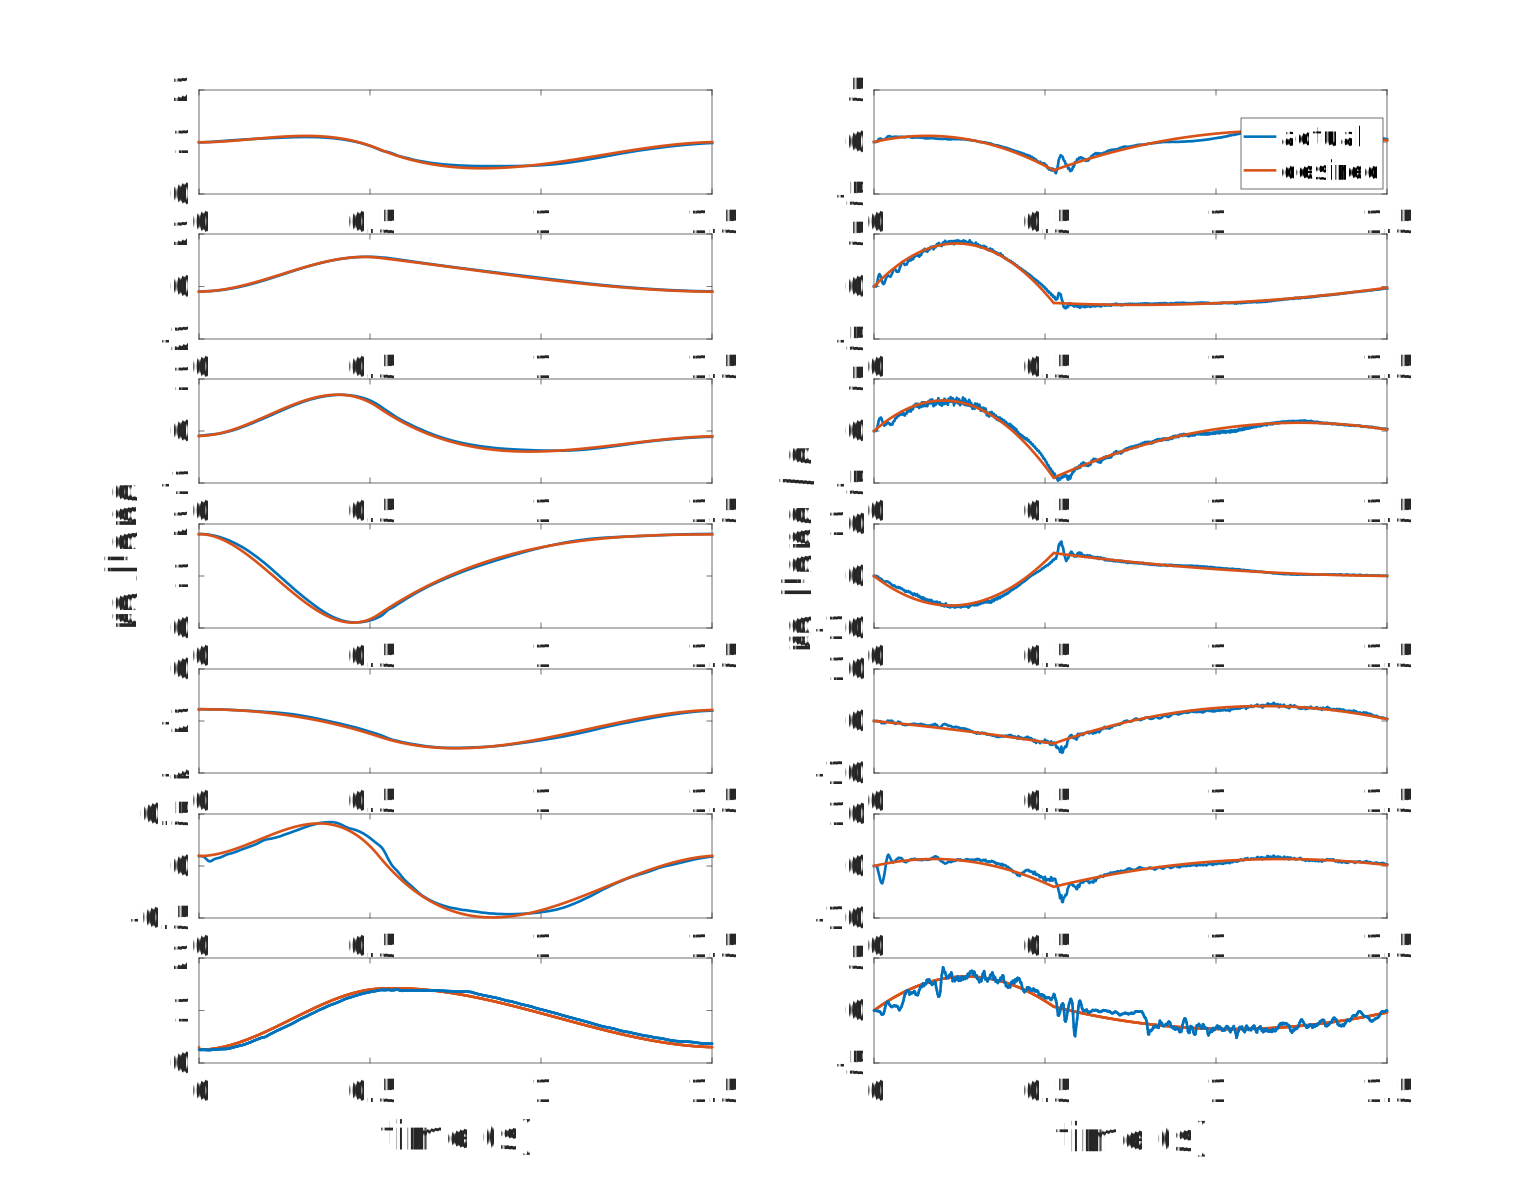
\includegraphics[scale=0.20]{act_vs_des_joints.pdf}
  	\caption{Tracking errors are shown for each joint. The desired joint positions and velocities are tracked with a PD controller. The deviation from the desired hitting point, shown as an orange dot in Figure~\ref{exampleTT}, was for this example within three centimeters of the racket centre, resulting in a hit.}
  	\label{control-error}
\end{figure}
%
% EXPERIMENTS - SHOWING IMPROVEMENT OVER PREVIOUS EXP